\section{学位论文,论文答辩,和毕业}
\label{sec.thesis_viva_graduation}

你想毕业吗?你想成为Doctor吗?那就赶快看这里吧!只要一篇一百多页的论文,毕业不是梦!\sout{(发癫结束)}

\subsection{官方流程和时间线}
\label{sec.official.flowchart}

正如本攻略的宗旨是官方资料的补充,首先请尽量熟读下图的官方毕业流程,里面的时间线、条件和顺序都是万分准确的。

\begin{figure}[H]
    \centering
    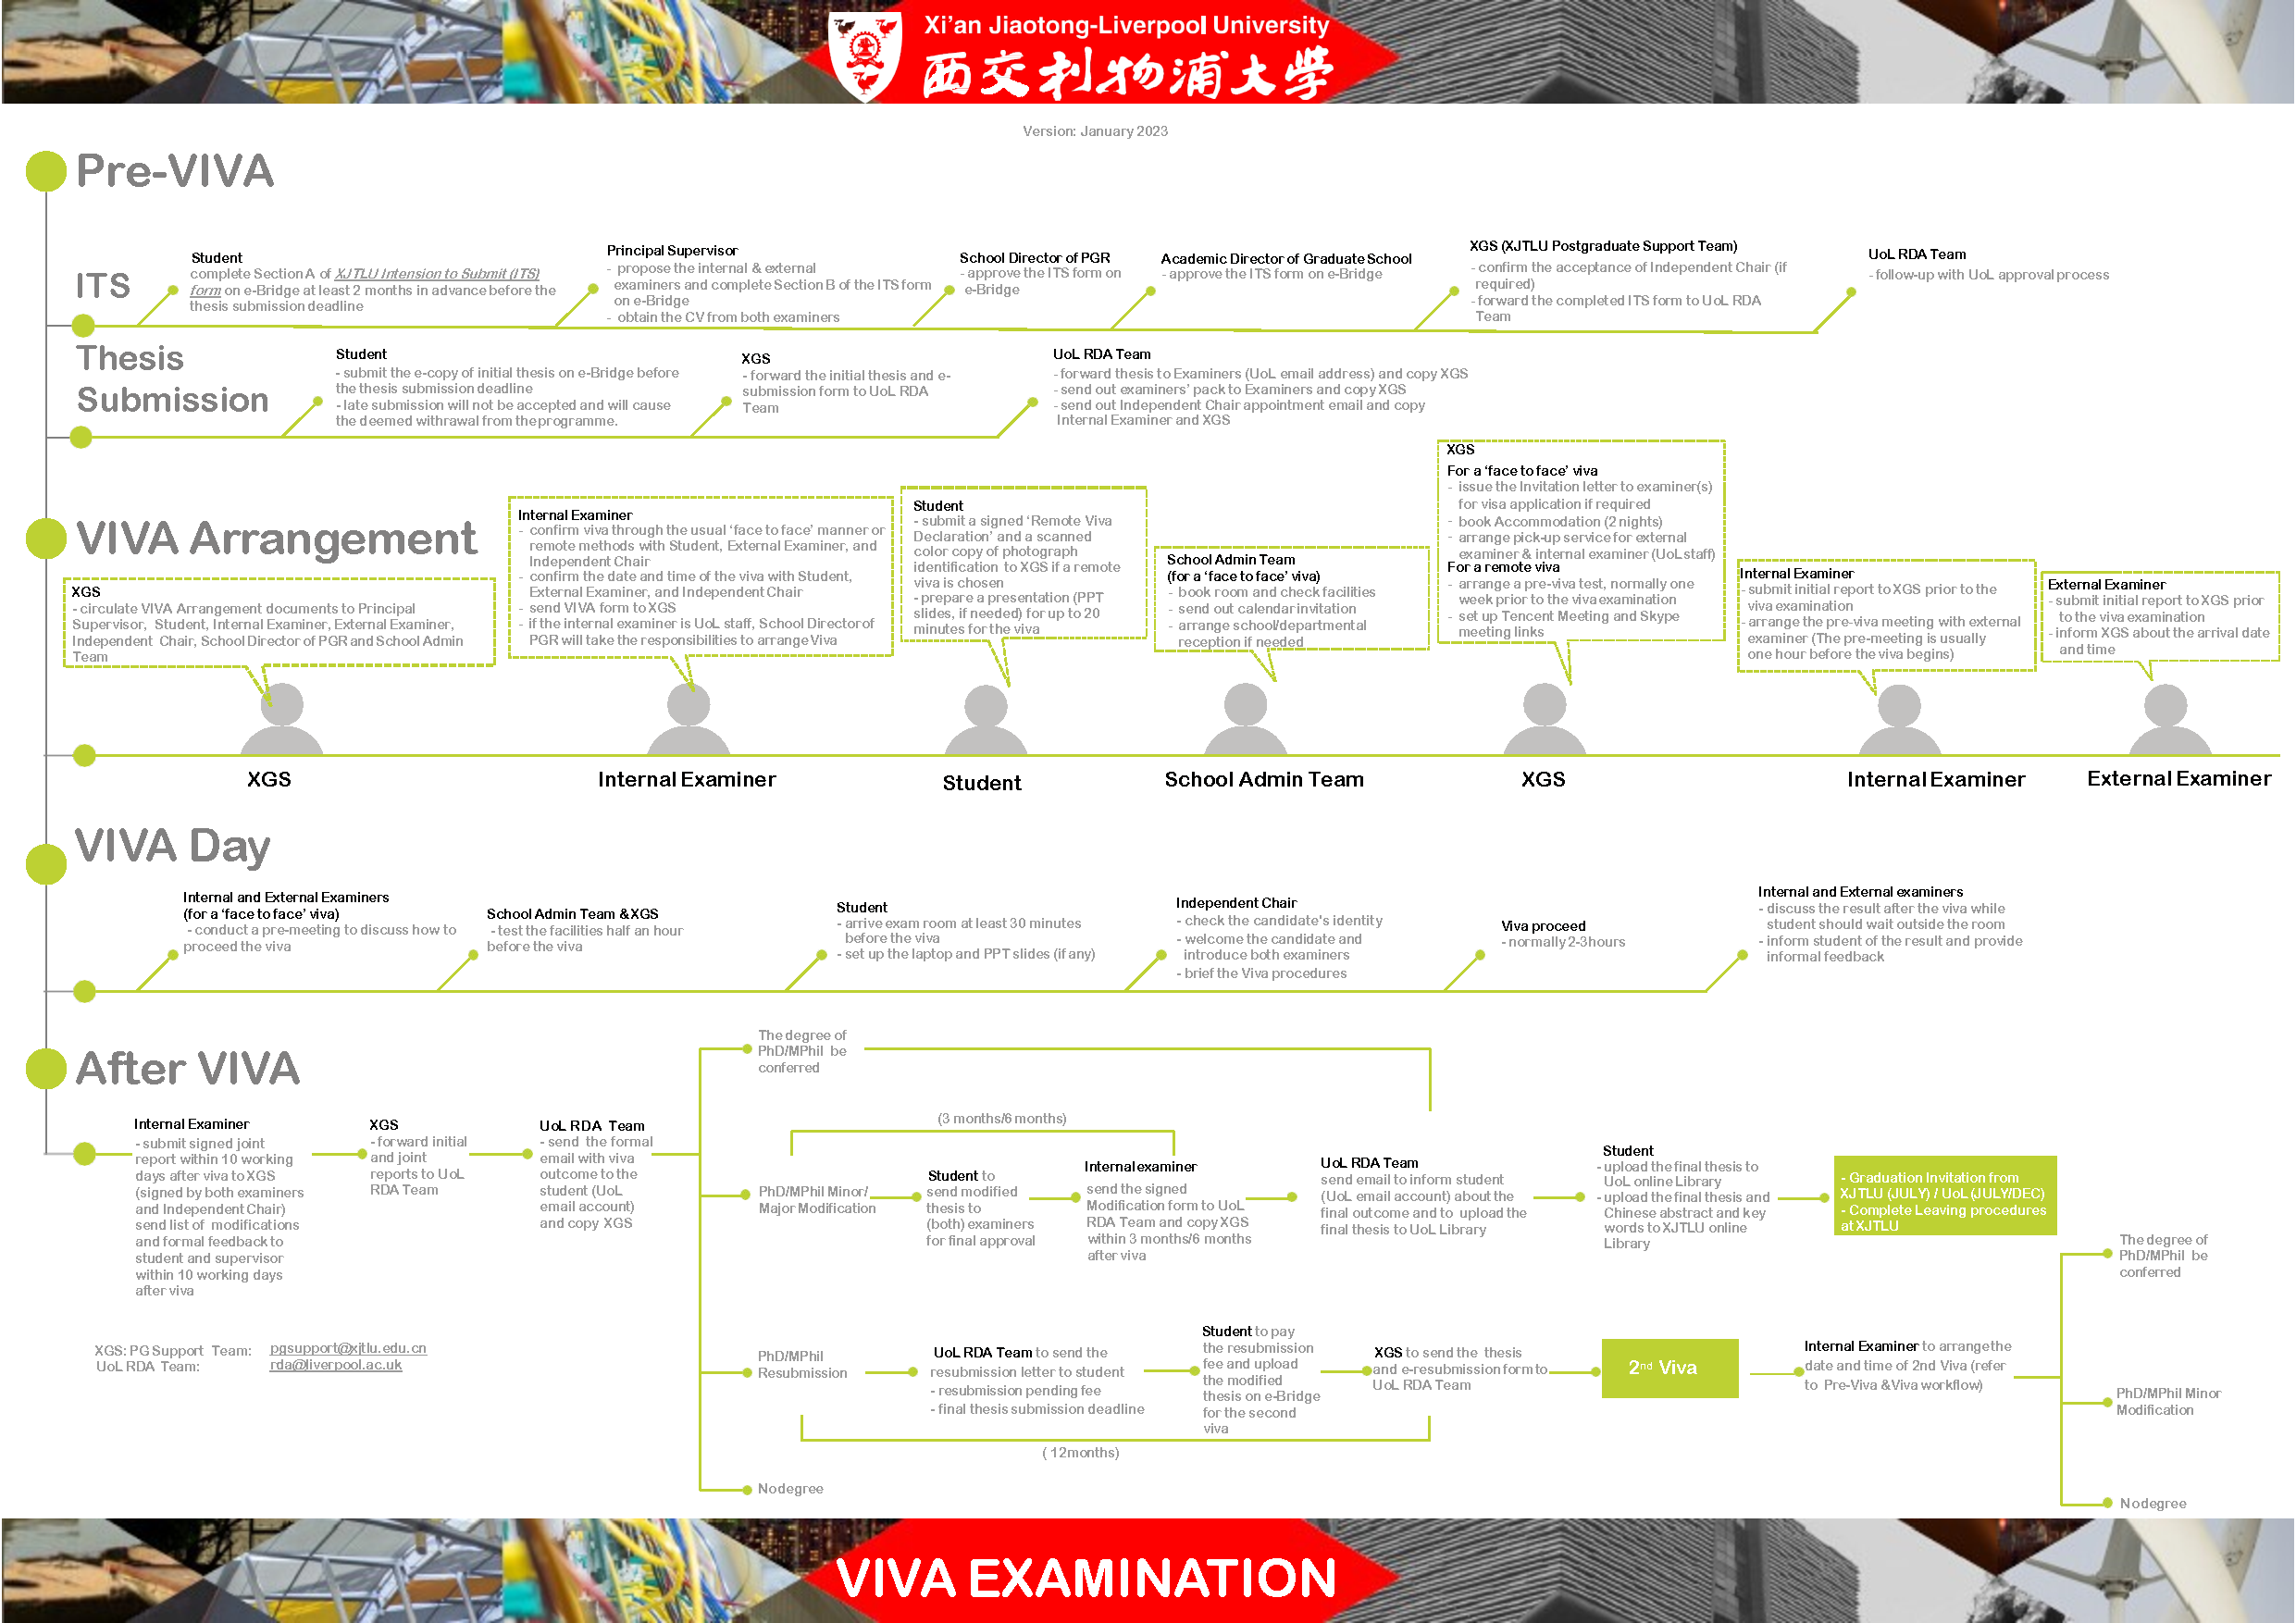
\includegraphics[width=\columnwidth]{fileshare/XJTLU VIVA Examination Arrangement Flowchart_2023.pdf}
    \caption{官方的毕业流程图。单独的文件可在fileshare里找到\url{https://gitee.com/kaiwu-astro/xp_pgrs_unofficial_guide/tree/main/fileshare}。注:我还真不知道这个文件在哪里下载的,这是我导发我的,想要最新版的可以在ebridge里找一下}
\end{figure}

如果想直到每个步骤大概要花多少时间,跳转章节 \ref{sec.graduation.time}。

\subsection{ITS: Intention to submit}

Q:ITS重要吗,我着急写论文呢,暂时不管它行不行

A:如果你对毕业时间有要求,请务必谨记尽早提交ITS表!ITS是你的论文和答辩一切程序的开始。现有规定,你的论文只能在\textbf{提交ITS之日起+2个月之后}才允许提交,可以延后,但不允许提前。(ITS提交后,一年内必须交论文;和你本身的论文deadline共同作用,以早的那个为准)

Q:ITS里面会填什么

A:毕业论文的题目、毕业论文的摘要、基本个人信息。题目和摘要不需要是最终决定的版本,也就是后面可以改。

Q:那我随便起个题目和摘要,走个过场行不行啊

A:这个表的作用是:导师和研究生院会拿着这个标题和摘要去决定你的内审、外审。这个题目和摘要也会发给他们。因此,和最终版可以有修改,但是也要尽量准确的反映你这几年的研究。

Q:我还要问

A:先看看官方文件:\url{https://www.liverpool.ac.uk/aqsd/academic-codes-of-practice/pgr-code-of-practice/}

\subsection{Thesis: 学位论文/毕业论文}

\subsubsection{格式和排版}

官方文件:\url{https://www.liverpool.ac.uk/media/livacuk/tqsd/code-of-practice-on-assessment/annex-7.1-PGR-CoP.pdf}
<-- 一切对格式不确定的请以这个为准。下面是微信群里的一些日经问题。

Q:可以用什么软件写毕业论文?

A:根据上面的规定,利物浦对软件没有要求,也就是你想用什么都可以。常用的有:Microsoft Word, \LaTeX

Q:推荐用什么软件呢

A:\LaTeX 优点:(1)非常方便输入公式,(2)参考文献和引用处理起来非常方便,不需要Endnote等外部软件辅助,(3)格式美观,风格统一,排版很难难看,(4)文件小,文件可分散,方便备份。\LaTeX 缺点:学习成本较高。如果你们专业发期刊论文/会议论文都不用\LaTeX 而用Word,那你切换过来就要花些时间学习。

Q:上面这个排版要求文件要求好多好细,呜呜呜给我一份毕业论文模板吧呜呜呜呜

A:
\begin{enumerate}
    \item Word还真的有一个官方模板,可以在本项目fileshare下载\url{https://gitee.com/kaiwu-astro/xp_pgrs_unofficial_guide/tree/main/fileshare}。来源:ELC Thesis Writing Camp的老师
    \item \LaTeX 没有官方模板,但数理学院(SMP)的大部分毕业生都是用\LaTeX 写的毕业论文。可以直接在Overleaf模板库直接搜索Liverpool Thesis,应该只有一个搜索结果,采用即可。
    \item 请使用模板的同学特别注意,never fully trust the template! Word模板是西浦ELC的老师给的,不是利物浦给的;Overleaf更是民间模板。理论上,他们对你的论文和毕业都\textbf{不负责}。因此拿到模板过后,第一件事永远还是打开上面的Code of Practice,一条一条的比对看是否达到了要求。
\end{enumerate}

\subsubsection{字数}

Q:上面的CoD只说了一个字数上限,那最低字数要求呢?

A:另一个日经问题。我曾经在研究生院Thesis Writing Camp课程上问了老师,他的意见是,西浦Master thesis的字数上限是3w,因此PhD thesis最好超过这个数。但我后来发现不是这回事。我见过有的论文不到100页,有的接近200页,都毕业了。从全校来看,这个是真的没有要求。你如果不放心,还是想对最低字数有点数,很简单,去利物浦图书馆和西浦图书馆下载毕业论文,重点参考你们学院、你们系、你们专业、最好直接是你同门已毕业同学的毕业论文,有多少字有多少页。\textbf{请谨记,字数多并不能保证你能轻松毕业}。我的一个师兄thesis就是接近200页,吃了个大改,外审说他写得太多了像教科书。

\begin{flushright}
    (2024年08月12日 by \Wu)
\end{flushright}

\subsection{Thesis Defense}

\subsubsection{Pre- and Post-Defense Process}

\begin{enumerate}
    \item At least two months before officially submitting your thesis on e-bridge, have your supervisor select a list of potential examiners for your upcoming defense. Submit this list to XJTLU's pgsupport and the University of Liverpool for review and approval.
    \item After officially submitting your thesis on e-bridge, the university will contact the respective examiners and then reach out to you to confirm the defense date and format (the defense typically occurs within 1-3 months after submission. The format can be either online or offline — confirm specifics with pgsupport).
    \item Generally, there will be a rehearsal before the defense to test the network and PPT presentation. You can also request time to practice your presentation in the designated conference room.
    \item Before the defense, the examiners will hold an internal meeting, usually on the same day (though sometimes earlier). They will then invite you into the meeting room to officially start the defense. Besides the two (or three under special regulations) examiners, there will be an observer (responsible for overseeing the overall process, arranging breaks, and addressing any procedural questions you might have). During the formal defense, the observer typically does not speak. If you have any questions, feel free to ask them.
    \item After your PPT presentation, there will be a Q\&A session. Depending on the circumstances, this can last from 1.5 to 3.5 hours (historically, there have been instances lasting up to 7 hours). Once the Q\&A concludes, you will be asked to leave the room temporarily while the examiners deliberate. After about 10-15 minutes, you'll be invited back in and informed of the results.
    \item The examiners' revision report will be sent to you within 10 working days. Based on their feedback, you'll need to make the necessary revisions within the specified timeframe and submit them to the primary examiner for confirmation.
    \item Once everything is confirmed, upload the final version of your thesis to complete the process.
\end{enumerate}

\begin{flushright}
    July 5, 2024 by Ziwen Xie \\
    GPT translation proofread by \Shiyao
\end{flushright}

\subsubsection{How to Prepare for a Viva}

Experience from the School of Science:

\textit{Try not to cram everything into a couple of days. Spreading out your preparation helps maintain a good state of mind daily, which is crucial for performing well during the actual defense.}

\textbf{1. Thoroughly read your thesis word by word as if you are a new reader, considering the following questions as you go:}
\begin{enumerate}
    \item Are any paragraphs unclear?
    \item Can you fully grasp and independently explain specific concepts?
    \item Do you understand the relationships and differences between chapters and the internal logic of the overall structure?
    \item Are you aware of the internal logic between sections within chapters and the sequence of experimental designs?
    \item What issues can each experiment address individually or collectively? What conclusions can be drawn from each major chapter?
    \item Do you fully understand the algorithms, models, and basic concepts cited from the literature? How are they connected to your core research objectives?
    \item Are there any previously unnoticed expression errors or chart inaccuracies that need correction?
    \item What is the purpose of your research? What motivated the choice of your methodology? How does it have advantages over other methods?
\end{enumerate}

\textbf{2. After organizing these points, analyze each chapter (including the abstract) in detail:}
\begin{enumerate}
    \item Can you summarize the background information in your own words?
    \item What does each subsection convey? Ensure consistency among subsections within a chapter.
    \item Highlight the key points or core logic of specific experiments or experimental designs.
    \item Understand the progression, parallelism, or other relationships and differences among experimental results (e.g., Experiment A demonstrates 'a', which serves as the foundation for Experiment B—this is progressive. If 'a' and 'b' are similar, then A and B are parallel).
    \item Justify the selection of experimental subjects and models (including why other related subjects or models weren't used).
    \item Based on your results, what future experiments could be pursued? (This may include why certain experiments weren't conducted, reasons for future experiments, potential outcomes of future experiments, foundational assumptions, and practical challenges—which explain why they weren't done in the current phase but were considered).
    \item Ensure the abstract includes key results and innovations.
\end{enumerate}

\textbf{3. Key Points for Preparing Your PPT and Viva:}
\begin{enumerate}
    \item Allocate 20 minutes into four sections: background introduction, experimental setup, experimental results, and conclusions—in approximately 5 minutes each. You can shorten the first three sections since the examiners have already read your thesis.
    \item Print your thesis and bring it with you to the defense. Take notes during the Q\&A session (this also gives you brief moments to compose yourself).
    \item Include essential figures and results in your PPT with concise descriptions.
    \item You don't need to discuss the challenges you faced or focus on future experiments or designs (examiners may ask about these, or you might mention them when answering questions). Depending on the situation, you can omit this from your PPT to save time.
    \item Ensure your PPT runs smoothly, and all text and images are clear. During practice sessions, simulate the actual presentation scenario as closely as possible.
    \item Remember to drink water during the defense—sip slowly and frequently. Eat some high-energy, easily digestible food beforehand. If you're not hungry, consider a chocolate bar or an energizing drink. Arrive early to familiarize yourself with the environment, which can help calm your nerves (and don't forget to visit the restroom beforehand).
    \item When answering questions, feel free to reference any part of your thesis. Some points in earlier chapters may connect with later ones or relate to future plans and final conclusions. If an examiner asks something you're unsure about or haven't considered, it's okay to admit it. Express your willingness to explore it further and ask for guidance or references in their feedback to assist with your revisions.
    \item Typically, each question and answer lasts about 3-5 minutes. With two examiners, handling around 20 questions each is substantial. Usually, the defense lasts between two to two and a half hours, with breaks in between (but once you're engaged, you might lose track of time).
\end{enumerate}

\textbf{4. Non-Thesis Related Questions:}
\begin{enumerate}
    \item How can artificial intelligence and ChatGPT inspire your research?
    \item Can your research be applied to other types of data, diseases, or fields? Why?
    \item What do you think are the shortcomings in your field?
    \item What is your biggest takeaway from your doctoral studies?
    \item If you had to do it all over again, would you still choose to pursue a Ph.D. and undertake this project?
\end{enumerate}
Tips: It seems the examiners are just curious and want a chat. Relax and answer accordingly. \textbf{Finally, according to data from a pgsupport staff member, there has never been a failed defense since our university was established. So, don't worry too much—just perform as you normally would. Good luck.}

\textbf{5. Ask your supervisors if they can help you anticipate potential questions. If time permits, see if they can arrange a mock viva for you (optional). It's also beneficial to consult recent graduates about their defense experiences, as certain aspects may change yearly.}

\begin{flushright}
    July 5, 2024 by Ziwen Xie \\
    GPT translation proofread by \Shiyao
\end{flushright}


\subsection{我想尽快拿学位证!如何速通毕业流程}

急急急,你就是急急国王。下面是一个合格的急急国王必须知道的事。

\subsubsection{毕业的证明文件}

\begin{enumerate}
    \item 完读证明(Completion of Studies Certificate),由西浦研究生院开具。证明内容:已提交毕业论文,已通过答辩,即将在XXXX年X月的毕业典礼上授予博士学位。我的Example:
    \begin{figure}[H]
        \centering
        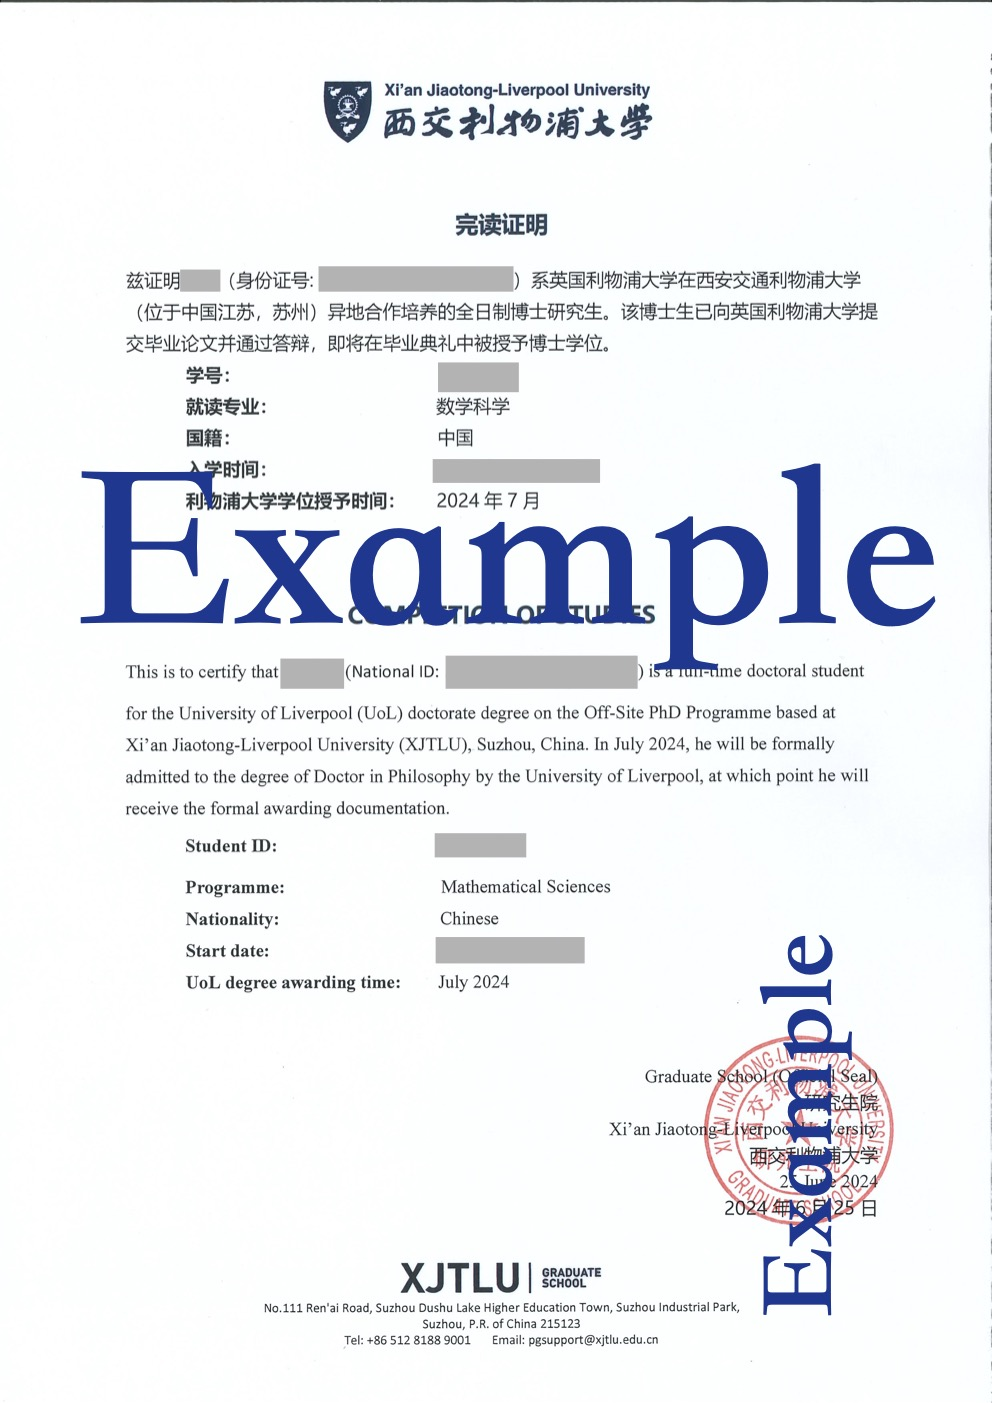
\includegraphics[width=0.8\columnwidth]{author-folder/Kai.Wu/Completion_of_Studies_Certificate_EXAMPLE.jpg}
        \caption{仅供参考,因此加上了巨大的example防止非法盗用}
    \end{figure}
    \item 学位证(aka PhD degree, degree certificate)。注意!利物浦规定,学位只会在\textbf{利物浦}毕业典礼上颁发,而利物浦毕业典礼一年只有两次,一般是7月某天和12月某天。如果你不去利物浦毕业典礼,会在毕业典礼前后先给学位证的电子版(有法律效力,可办中外合办认证),然后原件慢悠悠的邮寄到西浦。
    \item 中外合办学位认证。拿到电子学位证即可办理 \url{https://zwfw.cscse.edu.cn/}。持有该认证,你的利物浦学位就在中国境内被教育部承认。
\end{enumerate}

因此,首先确定你要去的公司/单位能接受哪种证明文件。最松的情况,你答辩完收到利物浦确认的Pass (with minor/major modification)邮件就行。也有能接受完读证明的。如果对方比较死板,不见学位证就不行,甚至没有中外合办认证也不行,那就要特别规划好毕业进度,因为每年只发2次证!

\subsubsection{学位证:最关键时间节点}

如果你确定不需要赶时间拿学位证,那本节接下来的都可以忽略,因为完读证明任何时候都可以开。

Q:我能否在7月/12月毕业?硬性要求是什么?

A:最好的方式是直接上利物浦网站查询,或者直接google liverpool phd graduation。过去几年的要求都是:在某个时间点之前,利物浦图书馆确认收到你的\sout{终极完全不改版的}最终论文。例如,如果要参加2024年7月15日的利物浦毕业典礼(在这一天颁发学位证,或邮寄),需要在2024年6月25日之前,利物浦图书馆确定收到了最终论文。这份论文是你的内外审都满意、同意的最终版。如何走到这一步?看下一节。

\subsubsection{每个步骤要等多久?如何预估时间?}
\label{sec.graduation.time}

以下完全基于已毕业同学的经验整理。新毕业的同学,请不吝赐教,补充你的真实案例。

以 \ref{sec.official.flowchart} 中提到的流程图来梳理:
\begin{enumerate}
    \item ITS:你提交过后其实就不用管了,专心写论文吧,剩下的都是导师和研究生院的活。背后的流程:i. 导师propose内审老师、外审老师; ii.研究生院审核,可能因为觉得这个老师和你利益相关等原因驳回其中的某人,然后你导师重新propose,直到研究生院满意为止,定下来内审外审人选各一个。在这个阶段,严格来说你直到论文提交都不能直到内外审老师是谁,导师需要保密,所以也不要\textbf{太}为难你导师去问是谁。
    \item 首次论文提交 到 论文答辩:(30天±30天)提交后,西浦研究生院(XGS)和利物浦学位办(RDA)会花两三个工作日简单处理下论文,发给内外审。\textbf{内审}一旦收到论文,就负责安排答辩时间。也就是说,你的答辩日期完全取决于你+内审+外审+独立主席(independent chair)都有空的某个时候(正常2-3小时)。因此,最早答辩日 = 论文交了过后三四个工作日;最晚答辩日则没有规定,找到四个人有空的时间为止。如果你赶时间,你能做的:(1)论文提交过后,尽早找你的内审,催ta安排日期;(2)把你论文提交过后一两个月的日程尽量腾空,不要因为自己的日程耽误答辩;(3)内外审一旦决定就不好更换,但独立主席容易换(有时会出现答辩一周前主席没空,找人另一老师顶上的事情),如果你们四个人里面是主席时间不合适导致拖很晚,尽早找你导师看能不能换主席。正常来说:交论文+60天=答辩 算非常慢的(但也有例子,据说是交论文前后不巧遇到了利物浦搞罢工)。一般会在+30天左右。
    \item 答辩完成 到 最终论文通过:(0 - 180天,典型为3-4周)。根据答辩结果不同这一步会有很大区别。(1) Pass (无条件) = 0天,论文初版即为最终版。(2) Pass with minor modification (小改),绝大部分同学都是这个结果。(3)Pass with major mofication(大改)(其他比较惨的情况很少,\sout{建议让导师和他举荐的examiner打一架})。如果是2或3,内外审会在10工作日(=2周)内出具书面的修改报告。这个过程个人建议不要催,他们要交的表和报告不少。之后就取决于你能多快改完论文。改完过后,按利物浦邮件指示,把改好的论文用指定的方式发给老师。这一步完全取决于你的内外审老师多久能respond,以及他们对你的修改是否满意。因为按照流程,如果不满意,他们有权让你改到他们满意为止。为了避免反复迭代,建议和导师反复斟酌新文本,争取一次搞定。这个版本的论文不会自动作为最终版,你可以在里面用颜色或者加粗标注修改过的地方,方便两位老师查阅。
    \item 最终论文通过 到 利物浦图书馆确认收到:(7天)这一步只是行政手续。在通过后,RDA会发邮件通知你上传最终论文(我的情况:内审老师告诉我[他们已告诉XGS和RDA修改版通过],过了4天收到上传通知),然后你将最终论文发送给利物浦,过几天(我的情况:2天)就收到利物浦图书馆正式通知邮件,论文成功上传。
    \item 实际还有一些手续,比如西浦会也让你上传一份到西浦图书馆,不知道是否会影响毕业,收到通知过后也最好尽早完成。
    \item 电子degree:具有法律效力的电子版degree会在你毕业典礼日期的前后几天内颁发。按照利物浦给你的邮件,在verify.liverpool.ac.uk里查询。
    \item 纸质degree:如果你人去利物浦参加毕业典礼,那就是现场领取。如果你不去,会在你毕业典礼日期后官方邮寄到西浦,等就完事了。我的情况:7月15日利物浦毕业典礼(人没去),纸质版7月30日寄到了研究生院。如果到时候人已经不在学校,可以委托研究生院邮寄(不推荐,丢件没法补,风险自担)。
\end{enumerate}

\begin{flushright}
    (2024年08月12日 by \Wu)
\end{flushright}